%\documentclass[spanish]{beamer}
\documentclass{beamer}
\usepackage{pgf,pgfpages}
%\pgfpagesuselayout{4 on 1}[letterpaper,landscape,border shrink=0.5in]
\usepackage{algorithm,algorithmic}
%\usepackage{algorithm,algorithmicx}
%\usepackage[noend]{algpseudocode}
\usepackage{listings}
\lstset{basicstyle=\ttfamily,
	showstringspaces=false,
	commentstyle=\color{red},
	literate={á}{{\'a}}1
	{ã}{{\~a}}1
	{é}{{\'e}}1
	{É}{{\'E}}1
	{ó}{{\'o}}1
	{í}{{\'i}}1
	{ñ}{{\~n}}1
	{¡}{{!`}}1
	{¿}{{?`}}1
	{ú}{{\'u}}1
	{Í}{{\'I}}1
	{Ó}{{\'O}}1
}

\usepackage{beamerthemesplit}
\usepackage{color}
\usepackage[utf8]{inputenc}
\usepackage[spanish]{babel}
%\usepackage[latin1]{inputenc}
%\usepackage[pdftex]{graphicx}
%\usepackage{algorithm}
%\usepackage{algorithmic-C}
%\usepackage{algorithmic}
\usepackage{amsthm}
\usepackage{multicol}
\usepackage{multirow}
\usepackage{fancyvrb,relsize}
\usepackage{hhline}
\usepackage{tikz}
\usetikzlibrary{trees, shapes, calc}
\newcommand{\inputTikZ}[2]{%
	\scalebox{#1}{\input{#2}}
}

\usetheme{Warsaw} %Gueno
%\usetheme{Darmstadt} %OK!
% \usetheme{Frankfurt} %OK!
%\usetheme{Goettingen}
%\usetheme{Dresden}
%\usetheme{JuanLesPins} %OK!!
%\usetheme{Marburg}
%\usetheme{Montpellier}
%\usetheme{Rochester} %sobrio
%\usetheme{Singapore}
%\usetheme{Szeged}

%\usecolortheme{albatross}
%\usecolortheme{seahorse}
%\usecolortheme{beetle}
%\usecolortheme{crane}
%\usecolortheme{dolphin}
%\usecolortheme{dove}
%\usecolortheme{fly}
%\usecolortheme{lily} %Gueno
\usecolortheme{orchid}%Gueno
%\usecolortheme{rose}
%\usecolortheme{seagull}
%\usecolortheme{whale}


\DefineVerbatimEnvironment%
      {VerbatimNN}%
      {Verbatim}%
      {fontsize=\relsize{-1}}
\DefineVerbatimEnvironment%
      {VerbatimNNN}%
      {Verbatim}%
      {fontsize=\relsize{-2}}

\DefineVerbatimEnvironment%
      {VerbatimPseudo}%
      {Verbatim}%
      {numbers=left, fontsize=\relsize{-1}}
\DefineVerbatimEnvironment%
      {VerbatimPseudoReduced}%
      {Verbatim}%
      {numbers=left, fontsize=\relsize{-2}}
\DefineVerbatimEnvironment%
      {VerbatimPseudoReduced2}%
      {Verbatim}%
      {numbers=left, fontsize=\relsize{-3}}
\DefineVerbatimEnvironment%
      {VerbatimC}%
      {Verbatim}%
      {commandchars=@ªº, numbers=left, fontsize=\relsize{-1}}
\DefineVerbatimEnvironment%
      {VerbatimReducedC}%
      {Verbatim}%
      {commandchars=@ªº, numbers=left, fontsize=\relsize{-2}}
\DefineVerbatimEnvironment%
      {VerbatimReduced2C}%
      {Verbatim}%
      {commandchars=@ªº, numbers=left, fontsize=\relsize{-3}}



%\AtBeginSubsection[]
%{
% \begin{frame}
% \frametitle{Sinopsis}
% Aqui decides: cada seccion y subseccion:
% \tableofcontents[currentsection,currentsubsection]
 %O solamente la seccion (Solo uno de ellos)
%\tableofcontents[currentsection]
% \end{frame}
%}

% Si quieres que todo por default aparezca de poco en poco
% descomenta esta linea
%\beamerdefaultoverlayspecification{<+->}

\setbeamertemplate{footline}{\hfill\insertframenumber/\inserttotalframenumber}
\setbeamertemplate{navigation symbols}{}

\setbeamercovered{transparent}

\title{ELO320 - Estructuras de Datos y Algoritmos\\Teoría de Grafos\\{\small Ruta más corta - Árbol de mínima expansión}}
%\subtitle{Ingeniería Civil Telemática UTFSM}
\author{Dr. Nicolás Gálvez R.\\{\small nicolas.galvez@usm.cl}}
\institute{Ing. Civil Telemática - Departamento de Electrónica}
\titlegraphic{
\includegraphics[scale=.14]{images/logoutfsm}}
\date{1er Semestre 2023}

\begin{document}

\frame{\titlepage}

%\section*{Sinopsis}
%\frame{  \frametitle{Sinopsis}\tableofcontents[pausesections]}
%
%

\section{Teoría de Grafos: Repaso}
\begin{frame}[fragile]
 \frametitle{¿Qué es un Grafo?}\small
Es un TDA que representa a un \textit{conjunto de objetos} los cuales pueden estar conectados mediante \textit{enlaces}. 

\begin{center}
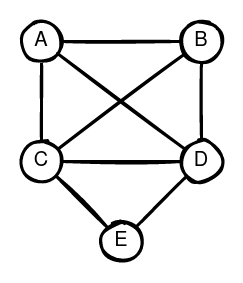
\includegraphics[width=0.3\linewidth]{images/graphs/graph-undirected}
\end{center}

Los grafos son fácilmente graficables, y en estos los objetos representados por nodos, llamados \textbf{vértices}, están interconectados enlaces denominados \textbf{aristas}.
\end{frame}

\begin{frame}[fragile]
 \frametitle{Formalización de Grafos}\small
Un grafo se define como una tupla $\mathcal{G} = (\mathcal{V}, \mathcal{A})$, en donde:
\begin{itemize}
\item $\mathcal{V}$: Es el conjunto de \textbf{vértices} o \textbf{nodos},
\item $\mathcal{A} = \{ (x,y)\ |\ (x,y) \in \mathcal{V}^2 \land x \neq y \}$: Es el conjunto de \textbf{aristas} o \textbf{enlaces}.
\end{itemize}

\begin{center}
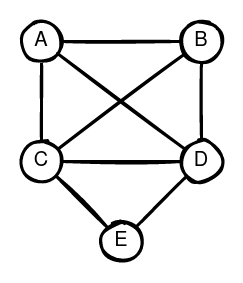
\includegraphics[width=0.3\linewidth]{images/graphs/graph-undirected}
\end{center}

Note que un arco $(x,y) \in \mathcal{A}$ conecta a dos nodos $x \in \mathcal{V} $ e $y \in \mathcal{V}$.
\end{frame}

\begin{frame}[fragile]
 \frametitle{Formalización de Grafos}
\small
Un grafo se define como una tupla $\mathcal{G} = (\mathcal{V}, \mathcal{A})$, en donde:
\begin{itemize}
\item $\mathcal{V} = \{A,B,C,D,E\}$.
\item $\mathcal{A} = \{(A,B), (A,C), (A,D), (B,C), (B,D), (C,D), (C,E), (D,E) \}$.
\end{itemize}
\begin{center}
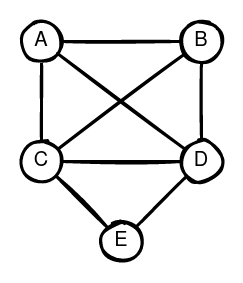
\includegraphics[width=0.3\linewidth]{images/graphs/graph-undirected}
\end{center}
\end{frame}

\section{Algoritmos de Optimización en Gráfos}
\begin{frame}[fragile]
 \frametitle{Algoritmos de Optimización en Gráfos}\small
\begin{itemize}
\item Ruta más Corta:
\begin{enumerate}
\item Algoritmo de Dijkstra.
\item Algoritmo de Bellmann-Ford.
\end{enumerate}
\item Árbol de mínima expansión:
\begin{enumerate}
\item Algoritmo de Prim.
\end{enumerate}
\end{itemize}
\end{frame}


\subsection{Ruta más corta}
\begin{frame}[fragile]
 \frametitle{Ruta más corta}\small
Imagine que ud. está jugando el famoso juego Pukamon GOES. Se encuentra en la ubicación A y en el resto de las posiciones hay un Pukamon diferente que ud. quiere atrapar. 
\begin{center}
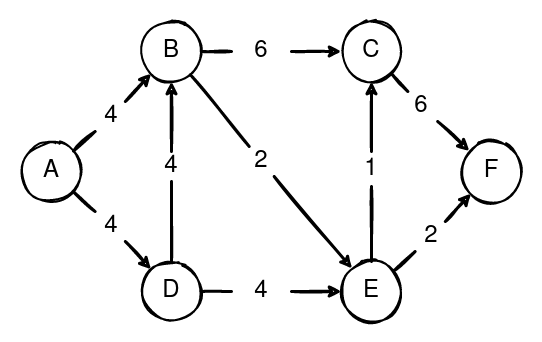
\includegraphics[width=0.5\linewidth]{images/graphs/dijkstra1}
\end{center}
\begin{itemize}
\item Si ud. trata de enumerar todos los caminos posibles, demorará mucho en encontrar una solución.
\item Ahora, imagine esta situación para 100, 1000 y 10000 ubicaciones distintas. Además, para 100, 1000 y 1000 enlaces.
\item ¿Cómo podemos afrontar este problema de forma eficiente para encontrar un óptimo para cada ruta?
\end{itemize}
\end{frame}

\begin{frame}[fragile]
 \frametitle{Ruta más corta}\small
Imagine que ud. está jugando el famoso juego Pukamon GOES. Se encuentra en la Posicion A y en el resto de las posiciones hay un Pukamon diferente que ud. quiere atrapar. 
\begin{center}
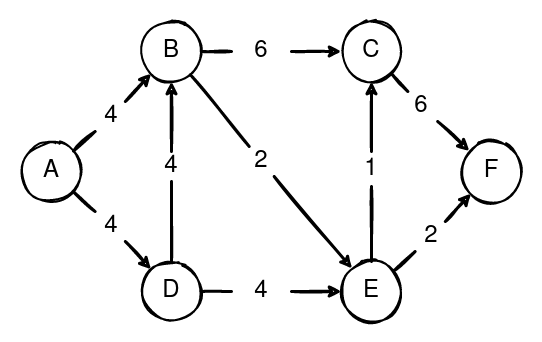
\includegraphics[width=0.5\linewidth]{images/graphs/dijkstra1}
\end{center}

Variantes:
\begin{itemize}
\item \textbf{Origen simple (1 a todos).}
\item Destino simple (todos a 1).
\item Par Origen-Destino (1 a 1).
\item Todos los pares (todos a todos).
\end{itemize}
\end{frame}

\begin{frame}[fragile]
 \frametitle{Algoritmo de Dijkstra}\small
Algoritmo que permite determinar la distancia más corta en un Grafo Ponderado Positivo. 
\begin{itemize}
\item Puede ser dirigido y no dirigido.
\item Puede ser Cíclico o Acíclico.
\item Los pesos solo pueden ser positivos. 
\item Original: $\mathcal{O}(|\mathcal{V}|^2)$.
\item Otras implementaciones: $\mathcal{O}((|\mathcal{A}|+|\mathcal{V}|) \log{|\mathcal{V}|})$, $\mathcal{O}(|\mathcal{A}|+ |\mathcal{V}| \log{|\mathcal{V}|})$. 
\end{itemize}
\end{frame}

\begin{frame}[fragile]
 \frametitle{Algoritmo de Dijkstra}\small
\begin{center}
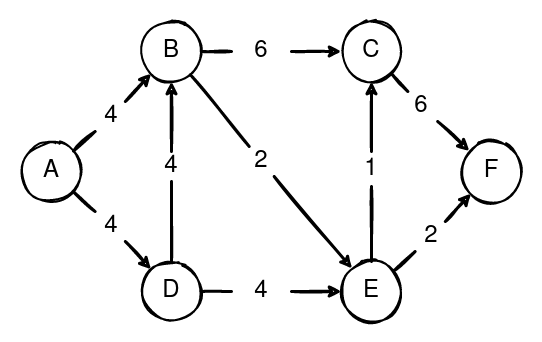
\includegraphics[width=0.75\linewidth]{images/graphs/dijkstra1}
\end{center}
\end{frame}

\begin{frame}[fragile]
 \frametitle{Algoritmo de Dijkstra}\small
\begin{center}
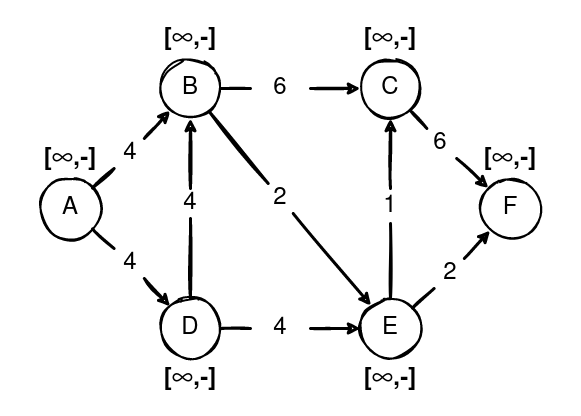
\includegraphics[width=0.75\linewidth]{images/graphs/dijkstra2}
\end{center}
\end{frame}

\begin{frame}[fragile]
 \frametitle{Algoritmo de Dijkstra}\small
\begin{center}
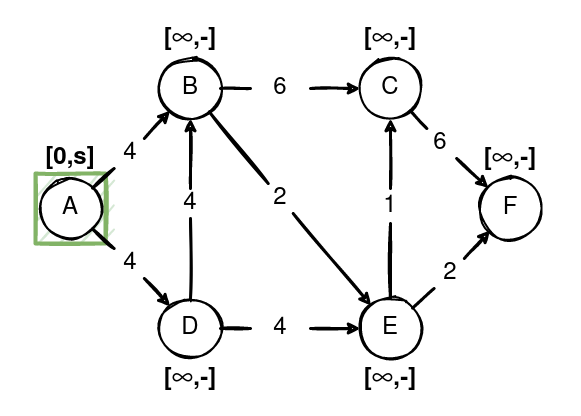
\includegraphics[width=0.75\linewidth]{images/graphs/dijkstra3}
\end{center}
\end{frame}

\begin{frame}[fragile]
 \frametitle{Algoritmo de Dijkstra}\small
\begin{center}
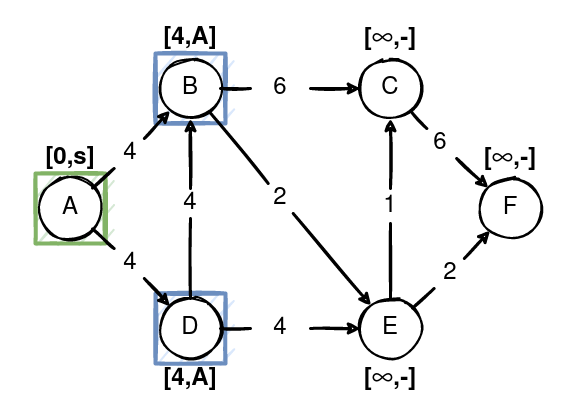
\includegraphics[width=0.75\linewidth]{images/graphs/dijkstra4}
\end{center}
\end{frame}

\begin{frame}[fragile]
 \frametitle{Algoritmo de Dijkstra}\small
\begin{center}
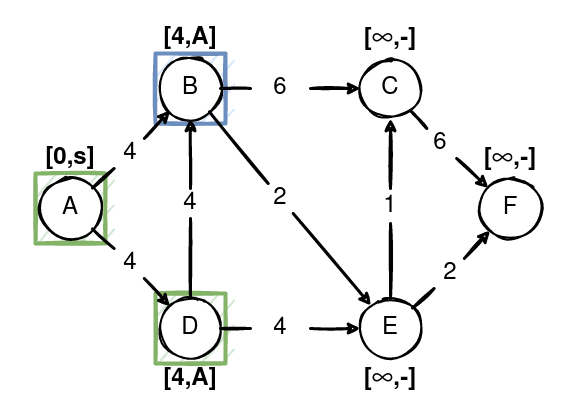
\includegraphics[width=0.75\linewidth]{images/graphs/dijkstra5}
\end{center}
\end{frame}

\begin{frame}[fragile]
 \frametitle{Algoritmo de Dijkstra}\small
\begin{center}
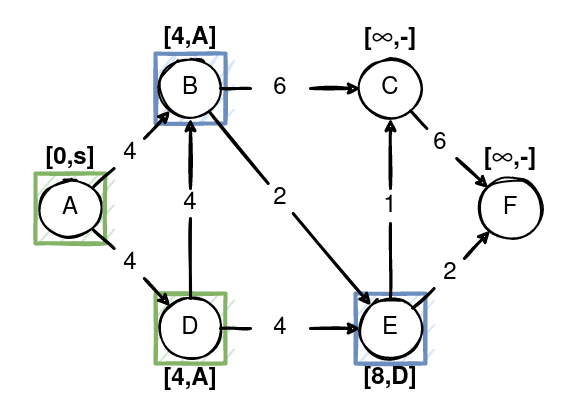
\includegraphics[width=0.75\linewidth]{images/graphs/dijkstra6}
\end{center}
\end{frame}

\begin{frame}[fragile]
 \frametitle{Algoritmo de Dijkstra}\small
\begin{center}
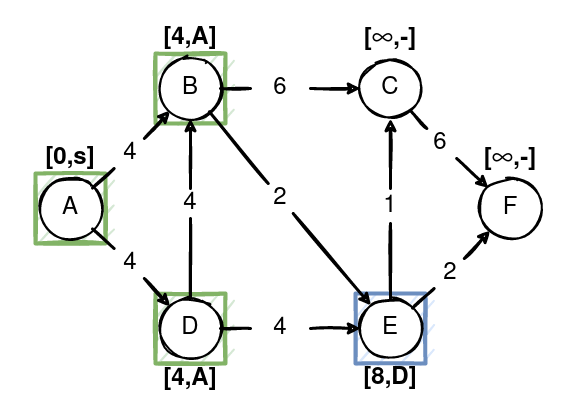
\includegraphics[width=0.75\linewidth]{images/graphs/dijkstra7}
\end{center}
\end{frame}

\begin{frame}[fragile]
 \frametitle{Algoritmo de Dijkstra}\small
\begin{center}
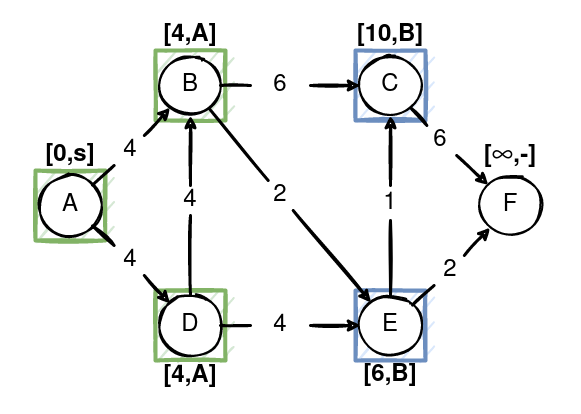
\includegraphics[width=0.75\linewidth]{images/graphs/dijkstra8}
\end{center}
\end{frame}

\begin{frame}[fragile]
 \frametitle{Algoritmo de Dijkstra}\small
\begin{center}
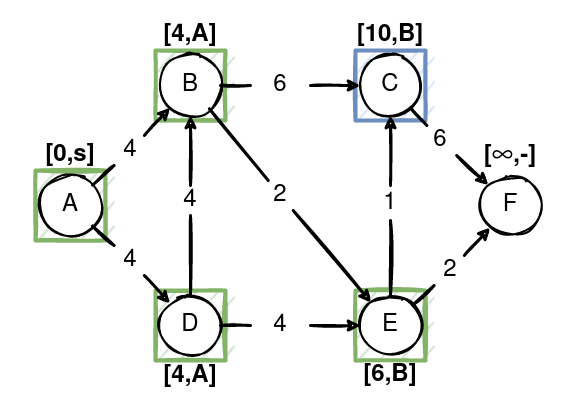
\includegraphics[width=0.75\linewidth]{images/graphs/dijkstra9}
\end{center}
\end{frame}

\begin{frame}[fragile]
 \frametitle{Algoritmo de Dijkstra}\small
\begin{center}
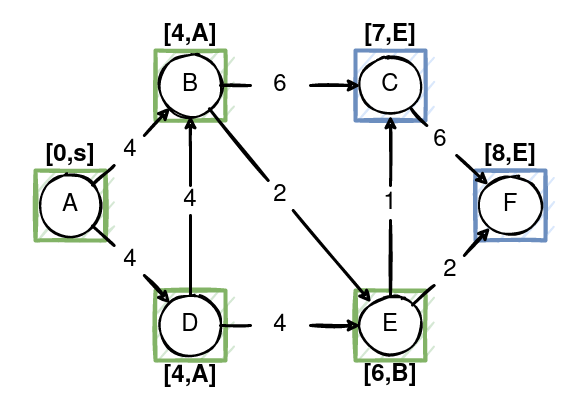
\includegraphics[width=0.75\linewidth]{images/graphs/dijkstra10}
\end{center}
\end{frame}

\begin{frame}[fragile]
 \frametitle{Algoritmo de Dijkstra}\small
\begin{center}
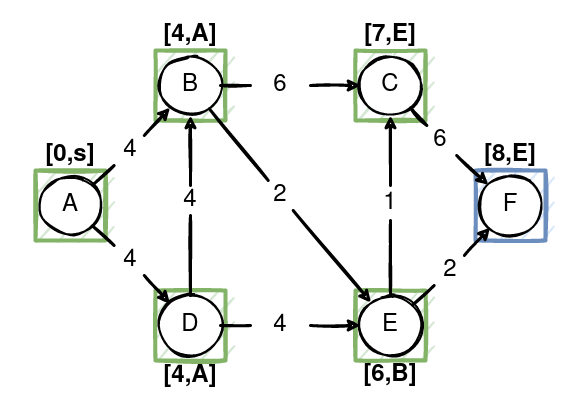
\includegraphics[width=0.75\linewidth]{images/graphs/dijkstra11}
\end{center}
\end{frame}

\begin{frame}[fragile]
 \frametitle{Algoritmo de Dijkstra}\small
\begin{center}
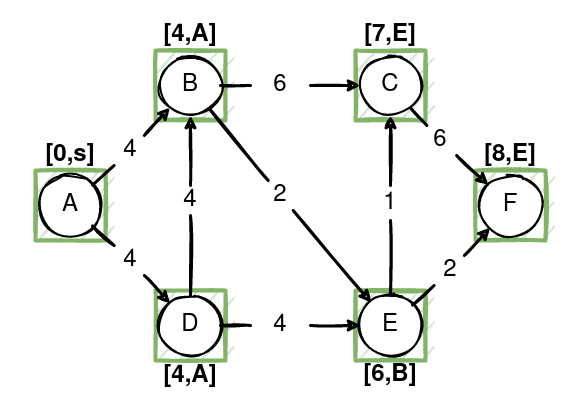
\includegraphics[width=0.75\linewidth]{images/graphs/dijkstra12}
\end{center}
\end{frame}

\begin{frame}[fragile]
 \frametitle{Algoritmo de Dijkstra}\small
\begin{center}
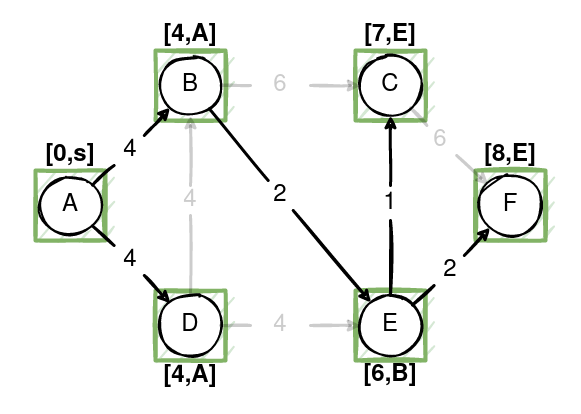
\includegraphics[width=0.75\linewidth]{images/graphs/dijkstra13}
\end{center}
\end{frame}

\begin{frame}[fragile]
 \frametitle{Algoritmo de Bellman-Ford}\small
Algoritmo iterativo basado en BFS que permite determinar la distancia más corta en un Grafo Ponderado. 
\begin{itemize}
\item Puede ser dirigido y no dirigido.
\item Puede ser Cíclico o Acíclico.
\item Los pesos pueden ser positivos y negativos. 
\item Menos eficiente que Dijkstra, pero más versátil.
\item Itera a lo más $|\mathcal{V}|-1$ veces. (cantidad de conexiones en óptimo).
\item $\mathcal{O}(|\mathcal{A}| \times |\mathcal{V}|)$.
\item Ejemplo: Primera iteración.
\end{itemize}
\end{frame}

\begin{frame}[fragile]
  \frametitle{Algoritmo de Bellman-Ford}\small
\begin{center}
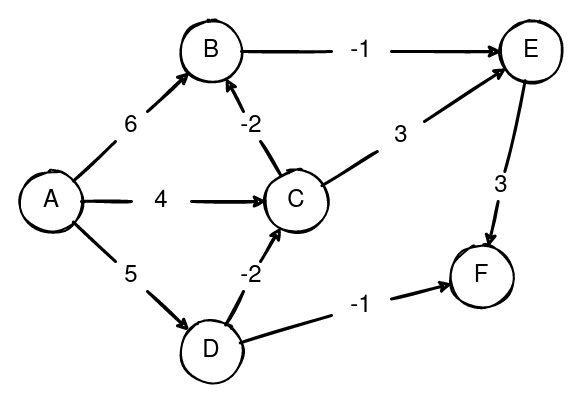
\includegraphics[width=0.75\linewidth]{images/graphs/bellmanford1}
\end{center}
\end{frame}

\begin{frame}[fragile]
  \frametitle{Algoritmo de Bellman-Ford}\small
\begin{center}
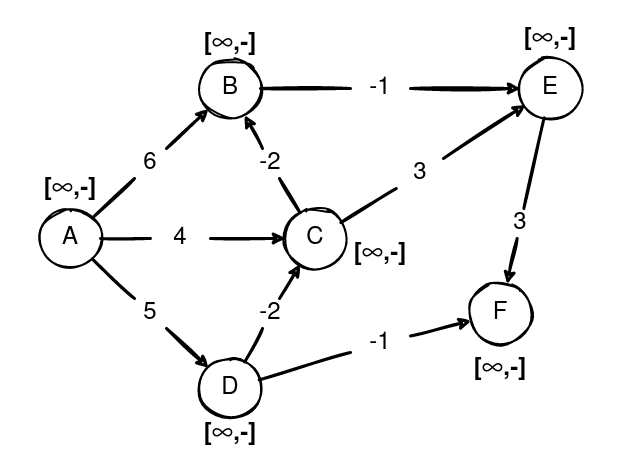
\includegraphics[width=0.75\linewidth]{images/graphs/bellmanford2}
\end{center}
\end{frame}

\begin{frame}[fragile]
  \frametitle{Algoritmo de Bellman-Ford}\small
\begin{center}
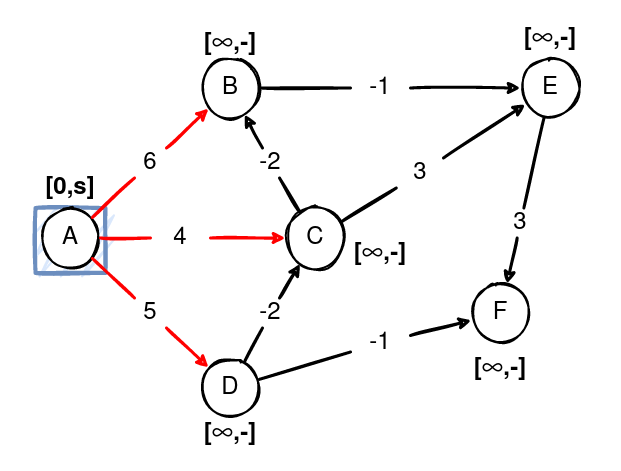
\includegraphics[width=0.75\linewidth]{images/graphs/bellmanford3}
\end{center}
\end{frame}

\begin{frame}[fragile]
  \frametitle{Algoritmo de Bellman-Ford}\small
\begin{center}
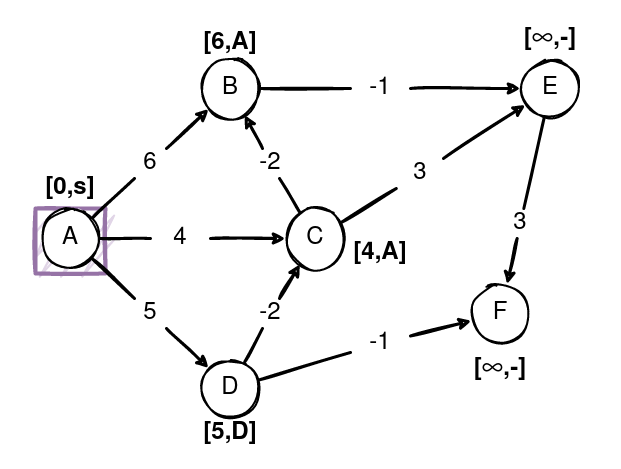
\includegraphics[width=0.75\linewidth]{images/graphs/bellmanford4}
\end{center}
\end{frame}

\begin{frame}[fragile]
  \frametitle{Algoritmo de Bellman-Ford}\small
\begin{center}
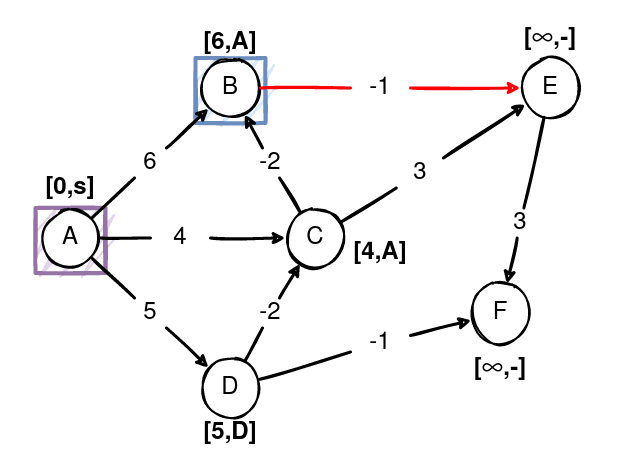
\includegraphics[width=0.75\linewidth]{images/graphs/bellmanford5}
\end{center}
\end{frame}

\begin{frame}[fragile]
  \frametitle{Algoritmo de Bellman-Ford}\small
\begin{center}
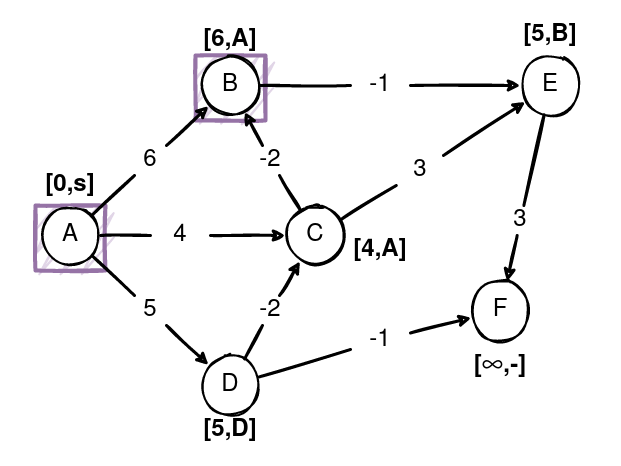
\includegraphics[width=0.75\linewidth]{images/graphs/bellmanford6}
\end{center}
\end{frame}

\begin{frame}[fragile]
  \frametitle{Algoritmo de Bellman-Ford}\small
\begin{center}
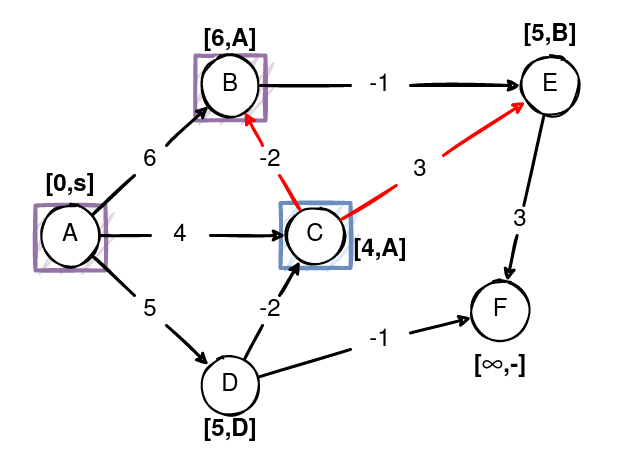
\includegraphics[width=0.75\linewidth]{images/graphs/bellmanford7}
\end{center}
\end{frame}

\begin{frame}[fragile]
  \frametitle{Algoritmo de Bellman-Ford}\small
\begin{center}
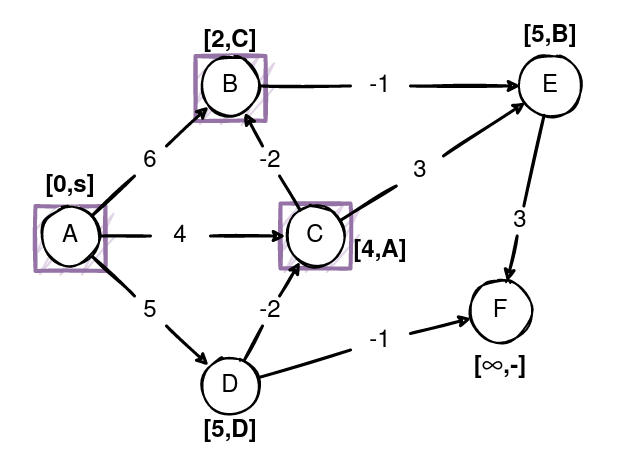
\includegraphics[width=0.75\linewidth]{images/graphs/bellmanford8}
\end{center}
\end{frame}

\begin{frame}[fragile]
  \frametitle{Algoritmo de Bellman-Ford}\small
\begin{center}
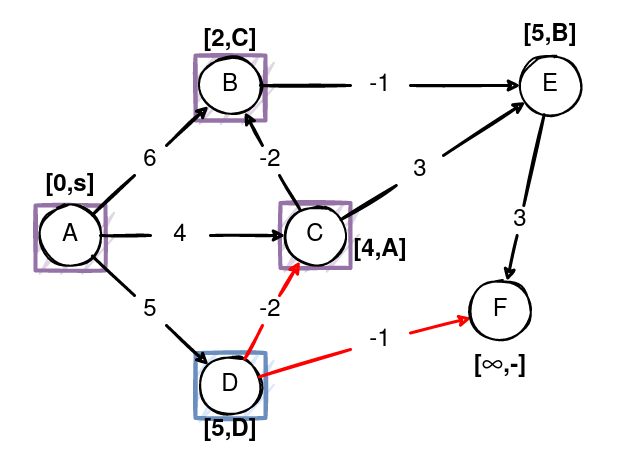
\includegraphics[width=0.75\linewidth]{images/graphs/bellmanford9}
\end{center}
\end{frame}

\begin{frame}[fragile]
  \frametitle{Algoritmo de Bellman-Ford}\small
\begin{center}
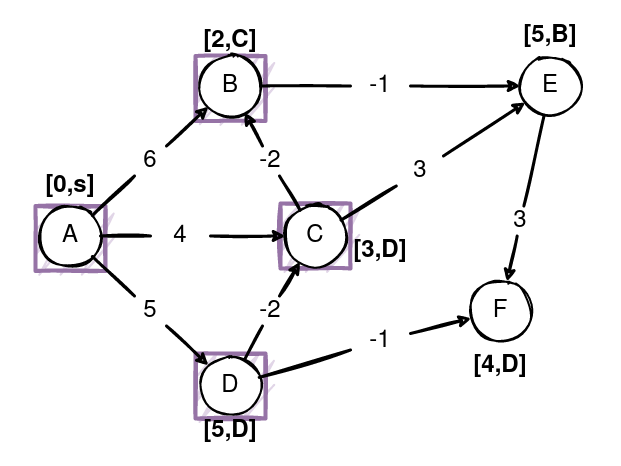
\includegraphics[width=0.75\linewidth]{images/graphs/bellmanford10}
\end{center}
\end{frame}

\begin{frame}[fragile]
  \frametitle{Algoritmo de Bellman-Ford}\small
\begin{center}
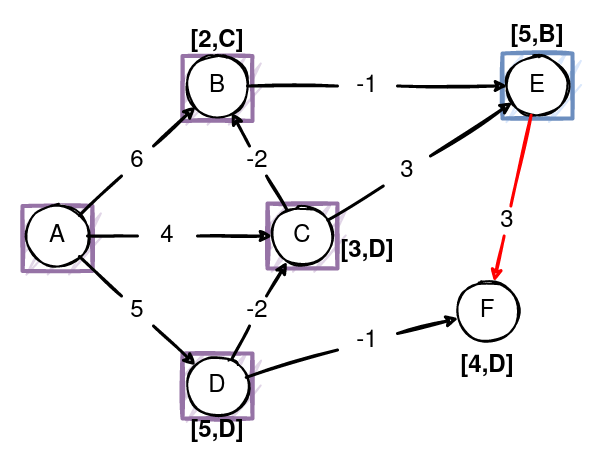
\includegraphics[width=0.75\linewidth]{images/graphs/bellmanford11}
\end{center}
\end{frame}

\begin{frame}[fragile]
  \frametitle{Algoritmo de Bellman-Ford}\small
\begin{center}
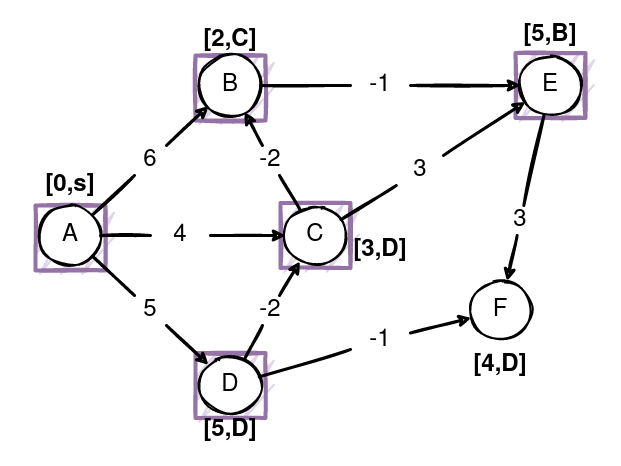
\includegraphics[width=0.75\linewidth]{images/graphs/bellmanford12}
\end{center}
\end{frame}

\begin{frame}[fragile]
 \frametitle{Algoritmo de Bellman-Ford}\small
\begin{center}
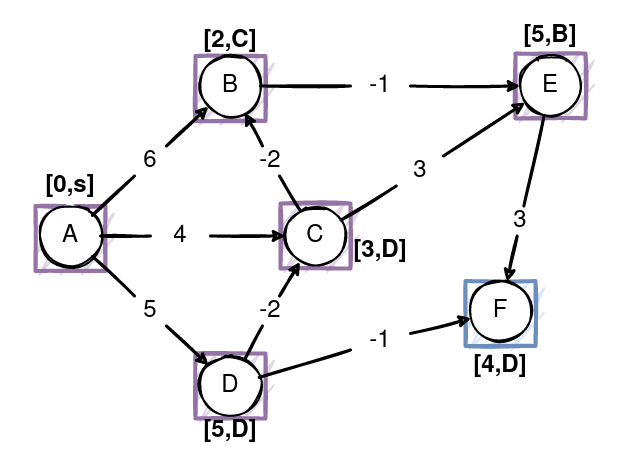
\includegraphics[width=0.75\linewidth]{images/graphs/bellmanford13}
\end{center}
\end{frame}

\begin{frame}[fragile]
 \frametitle{Algoritmo de Bellman-Ford}\small
\begin{center}
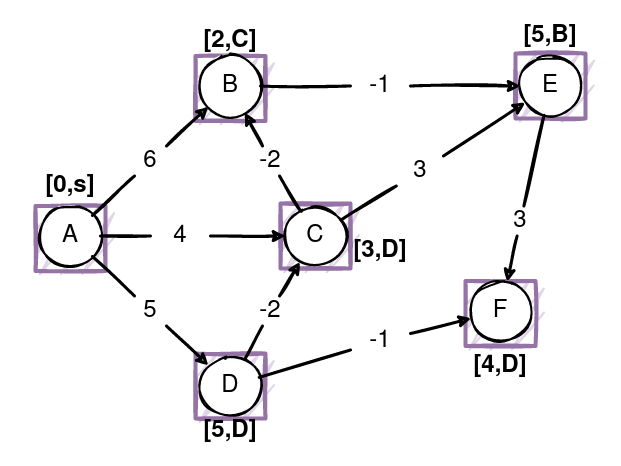
\includegraphics[width=0.75\linewidth]{images/graphs/bellmanford14}
\end{center}
\end{frame}

\begin{frame}[fragile]
 \frametitle{Algoritmo de Bellman-Ford}\small
\begin{center}
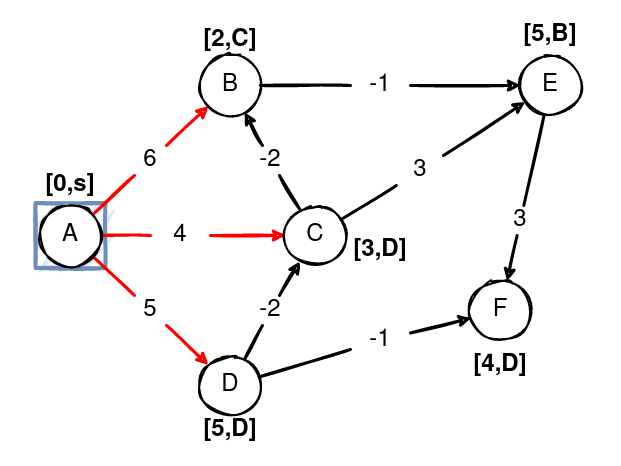
\includegraphics[width=0.75\linewidth]{images/graphs/bellmanford15}
\end{center}
\end{frame}


\subsection{Árbol de Mínima Expansión}
\begin{frame}[fragile]
 \frametitle{Árbol de Mímima Expansión}\small
Tal como vimos anteriormente, existen variados algoritmos de búsqueda en grafos que entregan árboles de expansión:
\begin{itemize}
\item BFS: Expansión mínima en grafos no ponderado.
\item DFS: Expansión en profundidad.
\item ¿Pero que hacer en el caso de grafos ponderdos?
\item Algoritmo de Prim.
\end{itemize}
\end{frame}

\begin{frame}[fragile]
 \frametitle{Árbol de Mímima Expansión}\small
Imagine que el ud. es programador del famoso juego LoT: League of TELegends, cuyo mapa se muestra en el siguiente grafo.

\begin{center}
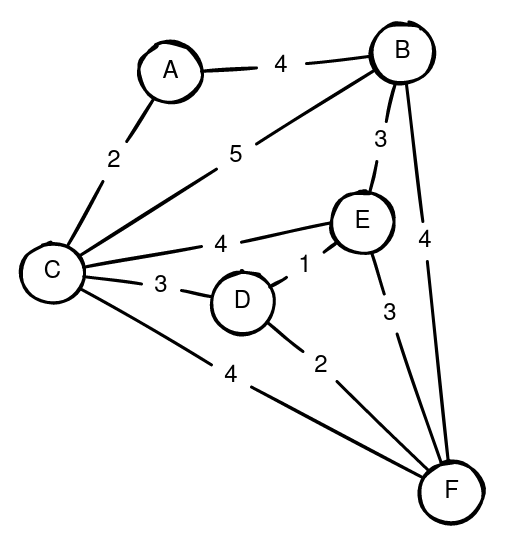
\includegraphics[width=0.4\linewidth]{images/graphs/prim1}
\end{center}

Debe programar el recorrido que deben seguir los soldados de infantería (minions) de su equipo desde la base ubicada en el nodo A hacia al resto de las ubicaciones de tal forma que el recorrido total sea mínimo, con el objetivo de sincronizar bien la salida periódica desde el origen (respawn).

\end{frame}


\begin{frame}[fragile]
 \frametitle{Algoritmo de Prim}\small
Algoritmo para encontrar el árbol de expansión mínima en un Grafo No Dirigido Ponderado. Falla con grafos dirigidos. 
\begin{itemize}
\item Debe ser no dirigido. 
\item Puede ser Cíclico o Acíclico.
\item Los pesos pueden ser positivos y negativos. 
\item Matriz de Adyacencia: $\mathcal{O}(|\mathcal{V}|^2)$.
\item Lista de Adyacencia: $\mathcal{O}((|\mathcal{A}|+|\mathcal{V}|) \log{|\mathcal{V}|})$
\item Otras implementaciones: $\mathcal{O}(|\mathcal{A}|+ |\mathcal{V}| \log{|\mathcal{V}|})$. 
\end{itemize}
\end{frame}

\begin{frame}[fragile]
 \frametitle{Algoritmo de Prim}\small
\begin{center}
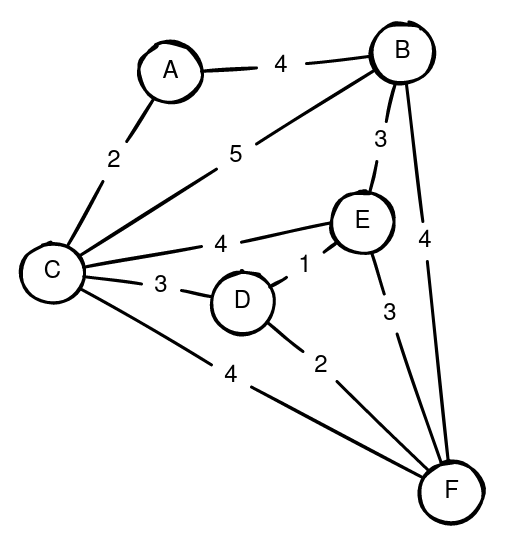
\includegraphics[width=0.6\linewidth]{images/graphs/prim1}
\end{center}
\end{frame}

\begin{frame}[fragile]
 \frametitle{Algoritmo de Prim}\small
\begin{center}
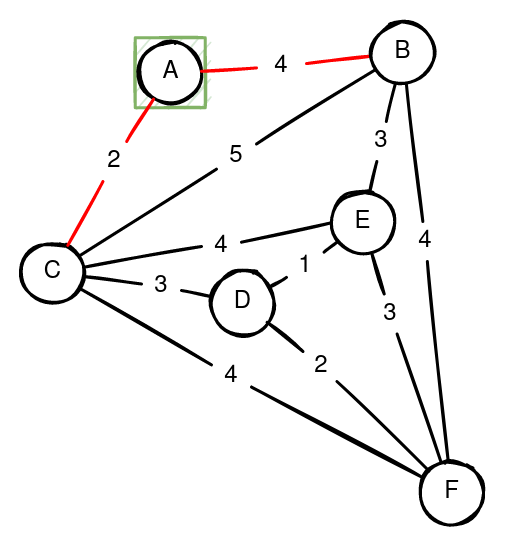
\includegraphics[width=0.6\linewidth]{images/graphs/prim2}
\end{center}
\end{frame}

\begin{frame}[fragile]
 \frametitle{Algoritmo de Prim}\small
\begin{center}
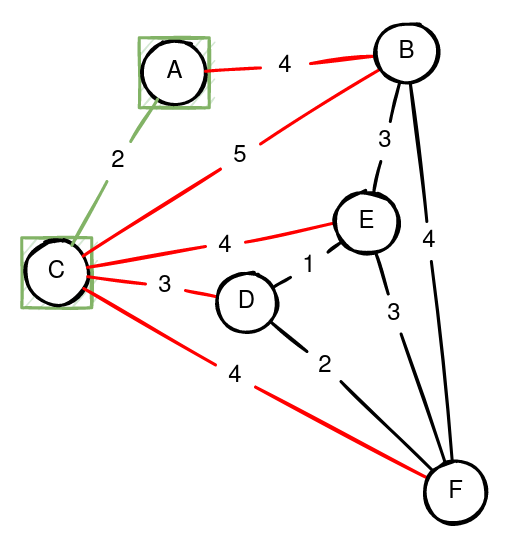
\includegraphics[width=0.6\linewidth]{images/graphs/prim3}
\end{center}
\end{frame}

\begin{frame}[fragile]
 \frametitle{Algoritmo de Prim}\small
\begin{center}
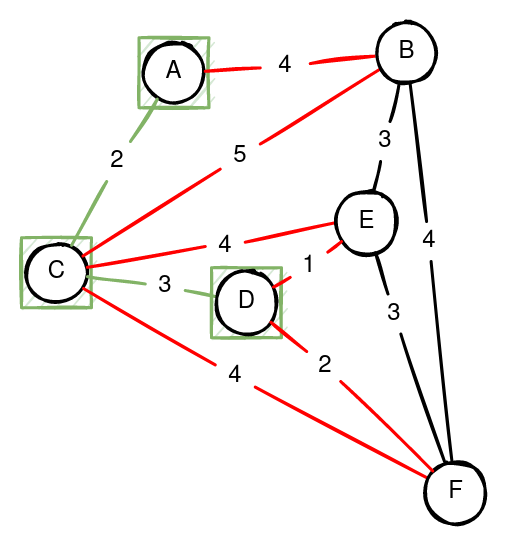
\includegraphics[width=0.6\linewidth]{images/graphs/prim4}
\end{center}
\end{frame}

\begin{frame}[fragile]
 \frametitle{Algoritmo de Prim}\small
\begin{center}
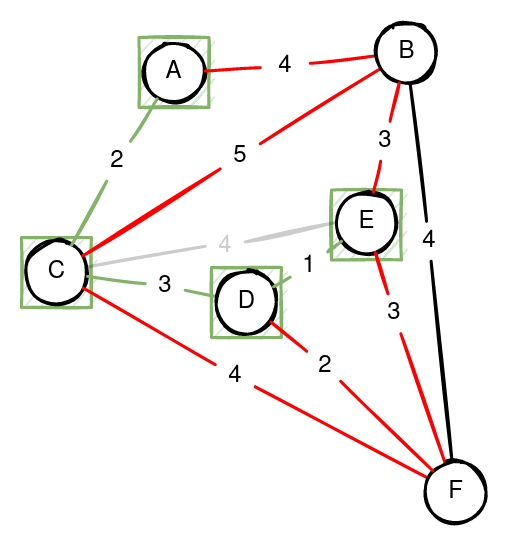
\includegraphics[width=0.6\linewidth]{images/graphs/prim5}
\end{center}
\end{frame}

\begin{frame}[fragile]
 \frametitle{Algoritmo de Prim}\small
\begin{center}
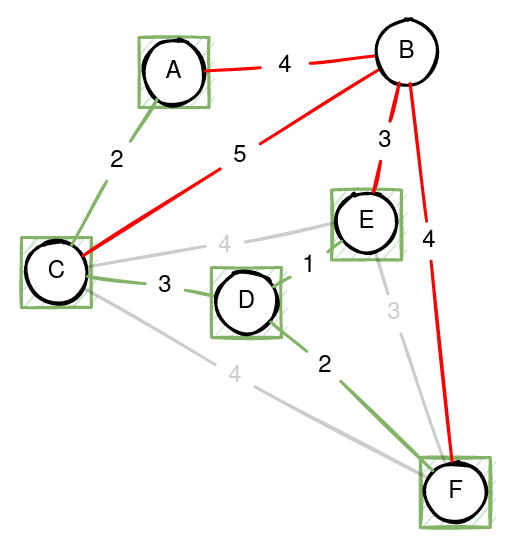
\includegraphics[width=0.6\linewidth]{images/graphs/prim6}
\end{center}
\end{frame}

\begin{frame}[fragile]
 \frametitle{Algoritmo de Prim}\small
\begin{center}
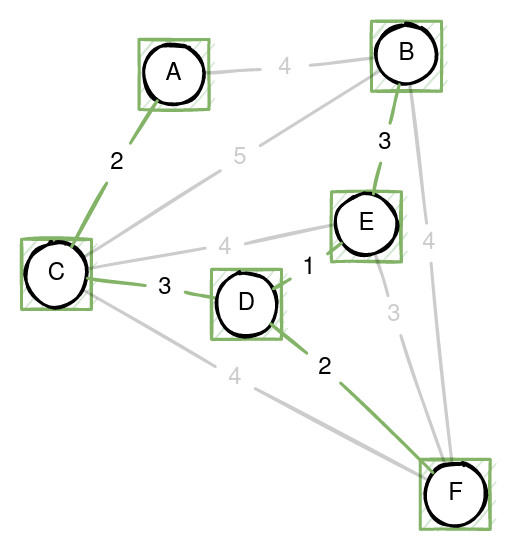
\includegraphics[width=0.6\linewidth]{images/graphs/prim7}
\end{center}
\end{frame}

\begin{frame}[fragile]
 \frametitle{Ejercicios}
\begin{itemize}
\item Aplique los tres algoritmos vistos en ésta clase al siguiente grafo:
\begin{center}
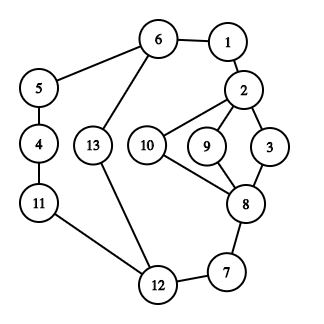
\includegraphics[width=0.5\linewidth]{images/graphs/example}
\end{center}
Suponga en los casos que ud. lo necesite, que puede direccionar el grafo a su conveniencia. 
\end{itemize}
\end{frame}

\begin{frame}[fragile]
 \frametitle{Fin del Curso}\small
\begin{lstlisting}
if(feof(ELO320)){
	printf("Hemos llegado al final del curso\n");
	exit(-1);
}
\end{lstlisting}
\end{frame}


\end{document}
